

\section{Aircraft Propeller}
An aircraft’s propeller consists of a rigid hub of radius $R$ and a flexible tapered blade of length $3R$ that has density $\rho (kg/m^3)$. The propeller is rotating about the center of the hub with a steady angular velocity $\omega$, thereby creating an effective axial distributed force in the blade. Neglect forces due to gravity. The cross sectional area distribution of the blade is $A(r)$, defined as

\begin{equation*}
    \input{q1/test}, \quad \text{if}\ R < r< 4R
\end{equation*}

\begin{figure}[h]
    \centering
    

\tikzset{every picture/.style={line width=0.75pt}} %set default line width to 0.75pt        

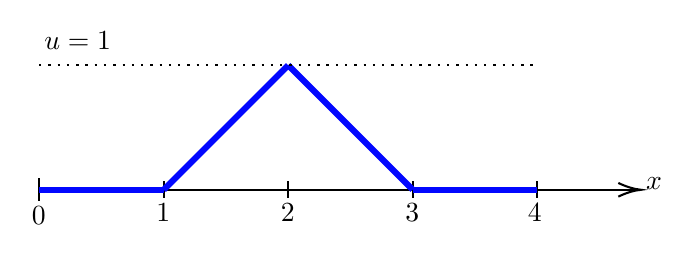
\begin{tikzpicture}[x=0.75pt,y=0.75pt,yscale=-1,xscale=1]
%uncomment if require: \path (0,300); %set diagram left start at 0, and has height of 300

%Straight Lines [id:da7588090942261074] 
\draw    (170,140) -- (458,140) (230,136) -- (230,144)(290,136) -- (290,144)(350,136) -- (350,144)(410,136) -- (410,144) ;
\draw [shift={(460,140)}, rotate = 180] [color={rgb, 255:red, 0; green, 0; blue, 0 }  ][line width=0.75]    (10.93,-3.29) .. controls (6.95,-1.4) and (3.31,-0.3) .. (0,0) .. controls (3.31,0.3) and (6.95,1.4) .. (10.93,3.29)   ;
\draw [shift={(170,140)}, rotate = 180] [color={rgb, 255:red, 0; green, 0; blue, 0 }  ][line width=0.75]    (0,5.59) -- (0,-5.59)   ;
%Straight Lines [id:da5719850269486109] 
\draw [color={rgb, 255:red, 2; green, 7; blue, 255 }  ,draw opacity=1 ][line width=2.25]    (170,140) -- (230,140) ;
%Straight Lines [id:da39606160939166957] 
\draw [color={rgb, 255:red, 2; green, 7; blue, 255 }  ,draw opacity=1 ][line width=2.25]    (230,140) -- (290,80) ;
%Straight Lines [id:da34987570129962964] 
\draw [color={rgb, 255:red, 2; green, 7; blue, 255 }  ,draw opacity=1 ][line width=2.25]    (290,80) -- (350,140) ;
%Straight Lines [id:da07428450981597945] 
\draw [color={rgb, 255:red, 2; green, 7; blue, 255 }  ,draw opacity=1 ][line width=2.25]    (350,140) -- (410,140) ;
%Straight Lines [id:da3360506402216956] 
\draw  [dash pattern={on 0.84pt off 2.51pt}]  (170,80) -- (410,80) ;

% Text Node
\draw (171,62.4) node [anchor=north west][inner sep=0.75pt]    {$u=1$};
% Text Node
\draw (461,132.4) node [anchor=north west][inner sep=0.75pt]    {$x$};
% Text Node
\draw (165,146.4) node [anchor=north west][inner sep=0.75pt]    {$0$};
% Text Node
\draw (225,145.4) node [anchor=north west][inner sep=0.75pt]    {$1$};
% Text Node
\draw (285,145.4) node [anchor=north west][inner sep=0.75pt]    {$2$};
% Text Node
\draw (345,145.4) node [anchor=north west][inner sep=0.75pt]    {$3$};
% Text Node
\draw (404,145.4) node [anchor=north west][inner sep=0.75pt]    {$4$};


\end{tikzpicture}

\end{figure}
% Problem 1, a
%%%%%%%%%%%%%%%%%%%%%%%%%%%%%%%%%%%%%%%%%%%%%%%%%%%%%%%%%%%%%%%%%%%%%%%%%%%%%%%%%%%%%%%%%%%%%%%
\begin{enumerate}[label=\alph*., start = 1]
    \item Write down the expression for body force due to rotational acceleration. 
    
\end{enumerate}



\pagebreak
\pagestyle{fancy}
\restoregeometry



% Problem 1, b
%%%%%%%%%%%%%%%%%%%%%%%%%%%%%%%%%%%%%%%%%%%%%%%%%%%%%%%%%%%%%%%%%%%%%%%%%%%%%%%%%%%%%%%%%%%%%%%
\begin{enumerate}[label=\alph*., start = 2]
    \item In the 1D equilibrium equation derived in class, the area of cross section was constant. Show that the 1D equilibrium equation for the case of a changing cross sectional area is $\frac{d}{dr}(\sigma A) + fA = 0.$
\end{enumerate}

% Problem 1, c
%%%%%%%%%%%%%%%%%%%%%%%%%%%%%%%%%%%%%%%%%%%%%%%%%%%%%%%%%%%%%%%%%%%%%%%%%%%%%%%%%%%%%%%%%%%%%%%
\begin{enumerate}[label=\alph*., start = 3]
    \item  Write down the boundary conditions for the problem. 
\end{enumerate}

% Problem 1, d
%%%%%%%%%%%%%%%%%%%%%%%%%%%%%%%%%%%%%%%%%%%%%%%%%%%%%%%%%%%%%%%%%%%%%%%%%%%%%%%%%%%%%%%%%%%%%%%
\begin{enumerate}[label=\alph*., start = 4]
    \item Find the axial stress distribution, $\sigma(r)$
\end{enumerate}